% Graphical abstract for Environmental Modelling & Software: 13 cm x 5 cm (journal minimum 1328 x 531 px; readable at 5 x 13 cm).
% Same black-and-white style as Fig. 1 (figs/arch5.tex). Build: pdflatex graphical_abstract.tex; TIFF via pdftoppm -r 300 -tiff.
\documentclass[border=0pt]{standalone}
\usepackage{mathptmx}
\usepackage{tikz}
\usetikzlibrary{arrows.meta,calc}
\begin{document}
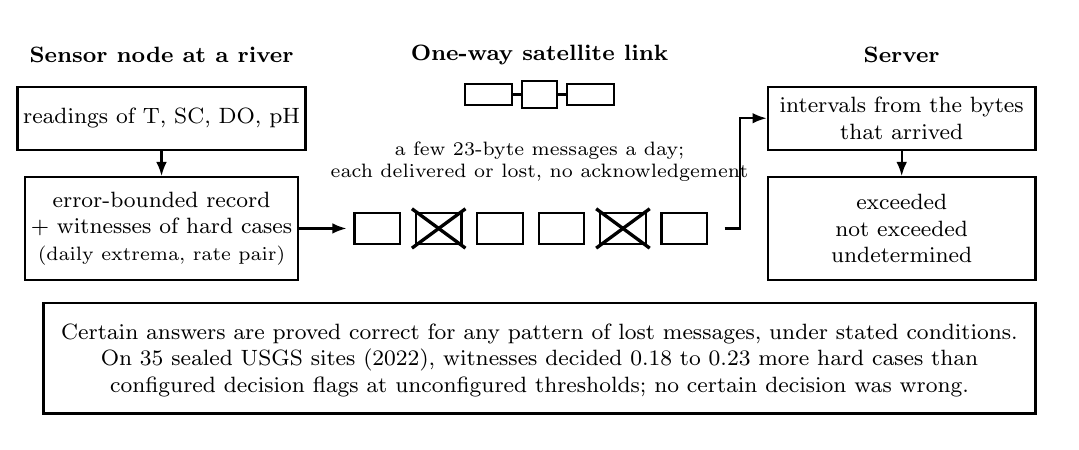
\begin{tikzpicture}[x=1cm, y=1cm,
  box/.style={draw, thick, align=center, fill=white, inner sep=2pt, font=\footnotesize},
  ttl/.style={font=\footnotesize\bfseries, align=center},
  arr/.style={-{Latex[length=1.8mm]}, thick},
  note/.style={font=\scriptsize, align=center}]
  \path[use as bounding box] (0,0) rectangle (13,5);

  % ---------------- node
  \node[ttl] at (1.7,4.65) {Sensor node at a river};
  \node[box, minimum width=3.0cm, minimum height=0.8cm] (sens) at (1.7,3.85) {readings of T, SC, DO, pH};
  \node[box, minimum width=3.0cm, minimum height=1.3cm] (enc) at (1.7,2.45) {error-bounded record\\+ witnesses of hard cases\\{\scriptsize (daily extrema, rate pair)}};
  \draw[arr] (sens) -- (enc);

  % ---------------- one-way link with lost messages
  \begin{scope}[shift={(6.5,4.15)}, thick]
    \draw[fill=white] (-0.22,-0.17) rectangle (0.22,0.17);
    \draw (-0.95,-0.13) rectangle (-0.35,0.13); \draw (0.35,-0.13) rectangle (0.95,0.13);
    \draw (-0.35,0) -- (-0.22,0); \draw (0.22,0) -- (0.35,0);
  \end{scope}
  \node[ttl] at (6.5,4.65) {One-way satellite link};
  \foreach \i/\lost in {0/0,1/1,2/0,3/0,4/1,5/0} {
    \pgfmathsetmacro{\xx}{4.15+0.78*\i}
    \draw[thick, fill=white] (\xx,2.25) rectangle ++(0.58,0.4);
    \ifnum\lost=1
      \draw[very thick] (\xx-0.05,2.2) -- ++(0.68,0.5);
      \draw[very thick] (\xx-0.05,2.7) -- ++(0.68,-0.5);
    \fi
  }
  \draw[arr] (enc.east) -- (4.05,2.45);
    \node[note] at (6.5,3.3) {a few 23-byte messages a day;\\each delivered or lost, no acknowledgement};

  % ---------------- server
  \node[ttl] at (11.1,4.65) {Server};
  \node[box, minimum width=3.4cm, minimum height=0.8cm] (know) at (11.1,3.85) {intervals from the bytes\\that arrived};
  \node[box, minimum width=3.4cm, minimum height=1.3cm] (out) at (11.1,2.45) {exceeded\\not exceeded\\undetermined};
  \draw[arr] (know) -- (out);
  \draw[arr] (8.85,2.45) -- (9.05,2.45) |- (know.west);

  % ---------------- result strip
  \draw[thick] (0.2,0.1) rectangle (12.8,1.5);
  \node[font=\footnotesize, align=center] at (6.5,0.775)
    {Certain answers are proved correct for any pattern of lost messages, under stated conditions.\\
     On 35 sealed USGS sites (2022), witnesses decided 0.18 to 0.23 more hard cases than\\
     configured decision flags at unconfigured thresholds; no certain decision was wrong.};
\end{tikzpicture}
\end{document}
